\section{Background}\label{sec:background}
Computer vision (CV) is a field of artificial intelligence that deals with the study of how computers can be made to gain high-level understanding from digital images or videos.
If AI allows the computer to think like a human as well as computer vision allows the computer to see like a human.

CV works like the human visual system, with the big difference in the fact that human uses year and year of experience to help the mind to understand what it is seeing.
As the biological neurons processes the information in the brain, the artificial neurons processes the information in the artificial neural network following the Hebbian plasticity (\cite{site:hebbian-plasticity}) rule: the connection between two neurons is strengthened if they are active at the same time.

In recent years, deep learning has revolutionized the CV field, achieving excellent results in many tasks, like: image classification, object detection, semantic segmentation, image captioning, image generation, etc.

The image classification task consists of assigning a label to an image with only one object (\hyperref[fig:figure-tulips]{Figure 1.1}).
\begin{figure}[H]
    \centering
    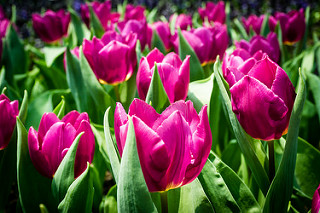
\includegraphics[width=0.8\textwidth]{images/1_1_tulips}
    \caption[Example of image classification]{Image classification: this image is classified as a tulip}
    \label{fig:figure-tulips}
\end{figure}
The object detection tasks consists of assigning a label and a bounding box to each object in the image.
The bounding box is a rectangle that encloses the object(\hyperref[fig:figure-object-detection]{Figure 1.2}).
\begin{figure}[H]
    \centering
    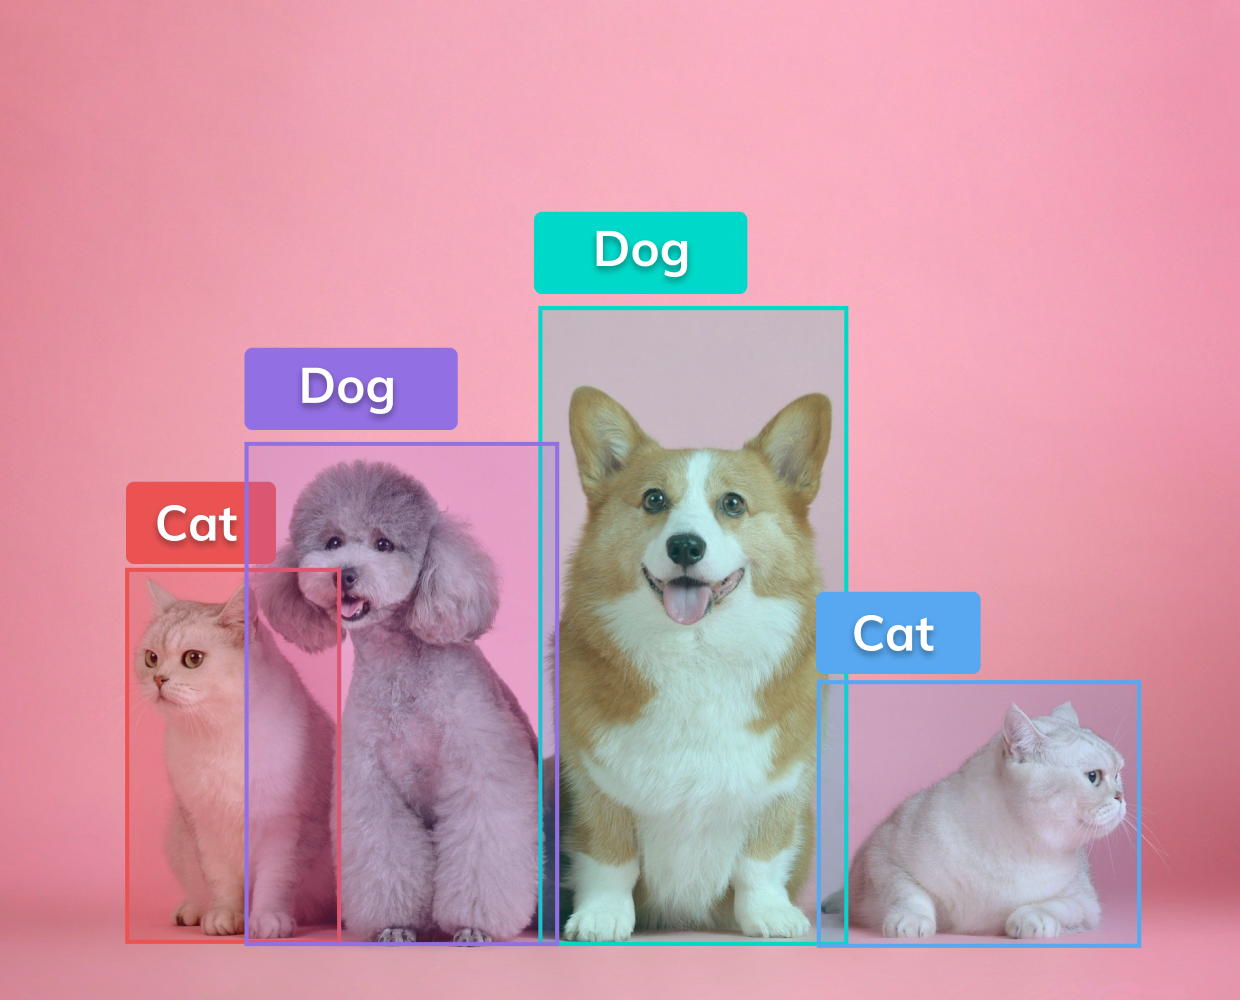
\includegraphics[width=0.8\textwidth]{images/1_1_object_detection}
    \caption[Example of object detection]{Object detection: this image contains two classes of objects, cat and dog.}
    \label{fig:figure-object-detection}
\end{figure}
The semantic segmentation task consists of assigning a label to each pixel of the image(\hyperref[fig:figure-semantic-segmentation]{Figure 1.3}).

\begin{figure}[H]
    \centering
    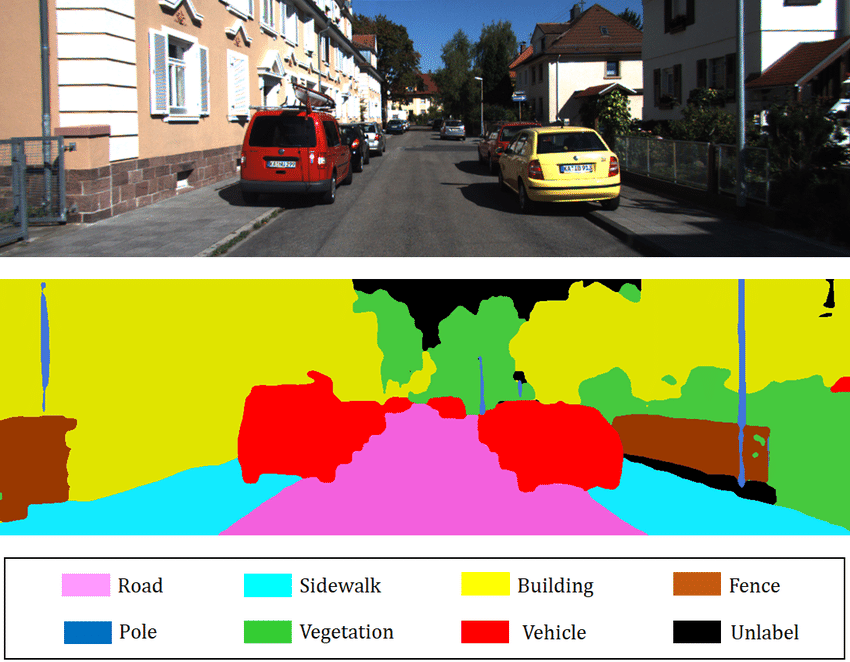
\includegraphics[width=0.8\textwidth]{images/1_1_semantic_segmentation}
    \caption[Example of semantic segmentation]{Semantic segmentation: each pixel is assigned a label.}
    \label{fig:figure-semantic-segmentation}
\end{figure}

Then, the modern CV systems can be used not only on the images, but also on video, like surveillance cameras to perform the real-time object detection and tracking, the most famous model is YOLOv3 (Redmon et al.~\cite{yolov3_paper}) (\hyperref[fig:figure-yolo-v3]{Figure 1.4}).

\begin{figure}[H]
    \centering
    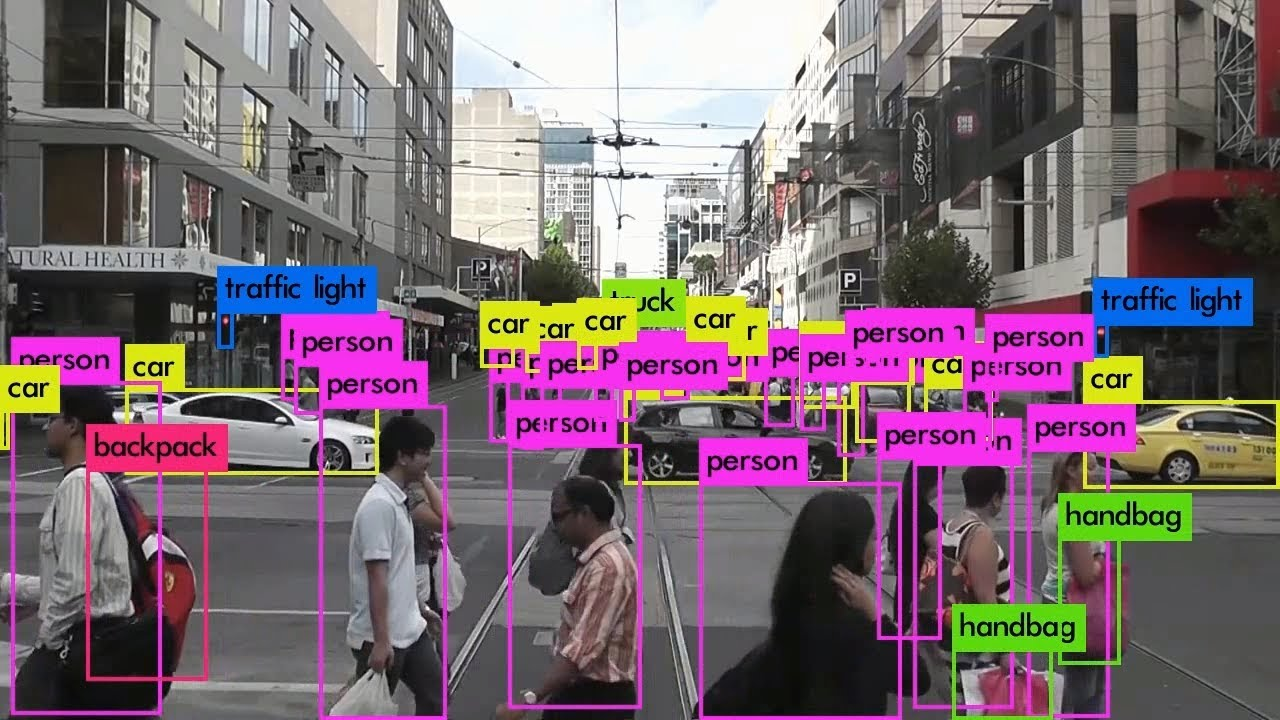
\includegraphics[width=0.8\textwidth]{images/1_1_yolov3}
    \caption{YOLO-V3 in action.}
    \label{fig:figure-yolo-v3}
\end{figure}

